\section{Tulemused}
\label{tulemused}

Selles peatükis esitatakse lamapuidu klassifitseerimis- ja segmenteerimismudelite kvantitatiivsed tulemused, mudelite otsinguprotsessi analüüs, valideerimine ja vigade uurimine. Peatükk jaguneb kaheks osaks: klassifitseerimismudelite arenduse ja lõplikud tulemused ning segmenteerimismudelite valideerimise tulemused.

\subsection{Klassifitseerimise tulemused}
\label{klassifitseerimise-tulemused}

\subsubsection{Käsitsi paanimärgistus ja automaatne filtreerimine}
\label{kasitsi-paanimargistus}

Klassifitseerimise andmestiku ettevalmistamise käigus märgistati pilootfaasis esimesed paanid käsitsi. Täiendavalt kasutati andmestiku mahu tõhusaks suurendamiseks loogikat, millega visuaalselt tühjad ja ilma lamapuiduta (näiteks puhta noorendiku või lageda maaga) paanid sildistati automaatselt negatiivseks. Pilootansambli hindamiseks saadi seeläbi kokku 21\,998 silti (sh 3\,380 lamapuiduga ja 18\,618 negatiivset paani). Neist 15\,850 kureeritud õppepaani suunati piloottreeningusse.

\subsubsection{Mudeliotsing ja arhitektuuride võrdlus}
\label{mudeli-otsinguprotsess}

Enne lõpliku ansambli ja prognoosimise juurde liikumist teostati laiendatud mudeliotsing mitmesuguste tehisnärvivõrkude arhitektuuri komponentide üle (19\,812 treeningpaani, 11 rasterikihti). Tabelist~\ref{tab:model-search-v1} järeldub, et CNN-Deep-Attn perekonna mudelid saavutasid üksikmudelitena testis kõige stabiilsemaid tulemusi. Samas demonstreeris virnaansambel asjaolu, et ansamblistrateegia annab antud ülesandes järjekindlalt parema tulemuse (F1-skoor 0,9672) kui parim üksikmudel (CNN-Deep-Attn-headwide: 0,9644).

\begin{table}[h!]
\centering
\caption{Parima mudeli otsingu tulemusnäitajad (19\,812 treeningpaani). Testvalimi tulemused põhinevad 2\,186 paanil; ${}^{\dagger}$ tähistab 5-kordse ristvalideerimise keskmist.}
\label{tab:model-search-v1}
\begin{tabular}{lllll}
\hline
\textbf{Mudel / ansambel} & \textbf{AUC} & \textbf{F1} & \textbf{Täpsus} & \textbf{Tagasikutse} \\
\hline
\multicolumn{5}{l}{\textit{Testvalimi tulemused}} \\
\hline
Virnaansambel (top-5)       & 0,9982 & 0,9672 & 0,9789 & 0,9558 \\
Pehme hääletus (top-5)      & 0,9982 & 0,9646 & 0,9646 & 0,9646 \\
CNN-Deep-Attn-headwide      & 0,9977 & 0,9644 & 0,9701 & 0,9587 \\
CNN-Deep-Attn               & 0,9973 & 0,9630 & 0,9673 & 0,9587 \\
CNN-Deep-Attn-headlight     & 0,9974 & 0,9614 & 0,9672 & 0,9558 \\
\hline
\multicolumn{5}{l}{\textit{Parimad alternatiivarhitektuurid, ristvalideerimine (${}^{\dagger}$)}} \\
\hline
ConvNeXt-small${}^{\dagger}$  & 0,9922 & 0,9546 & 0,9677 & 0,9420 \\
ConvNeXt-tiny${}^{\dagger}$   & 0,9935 & 0,9523 & 0,9626 & 0,9427 \\
EfficientNet-B2${}^{\dagger}$ & 0,9953 & 0,9493 & 0,9546 & 0,9440 \\
DenseNet-121${}^{\dagger}$    & 0,9912 & 0,9454 & 0,9640 & 0,9276 \\
\hline
\end{tabular}
\end{table}

\subsubsection{Pilootansambel ja paanide esmane hindamine}
\label{esialgse-ansambli-tulemused}

Tugevamate arhitektuuride selgumise järel moodustati neljamudeline pilootansambel (kolm \mbox{CNN-Deep-Attn} baasmudelit ja üks EfficientNet-B2), mis andis võimaluse skaleerida ennustusi aktiivõppe tarbeks. Esialgne märgistamisansambel saavutas testvalimil F1-skoori 0,9701 ja ROC AUC väärtuse 0,9987 (Tabel~\ref{tab:initial-ensemble}). Testiaegne andmerikastamine (TTA) põhine keskmistamine silus märgatavalt mudelite piiripealseid erinevusi.

\begin{table}[h!]
\centering
\caption{Esialgse pilootansambli üksikmudelite tulemusnäitajad valideerimisvalimil.}
\label{tab:initial-ensemble}
\begin{tabular}{llll}
\hline
\textbf{Mudel} & \textbf{Val AUC} & \textbf{Val F1} & \textbf{Otsustuslävi} \\
\hline
CNN-Deep-Attn (seeme 42) & 0,9969 & 0,9580 & 0,87 \\
CNN-Deep-Attn (seeme 43) & 0,9972 & 0,9570 & 0,81 \\
CNN-Deep-Attn (seeme 44) & 0,9974 & 0,9596 & 0,83 \\
EfficientNet-B2           & 0,9963 & 0,9463 & 0,72 \\
\hline
\textbf{Ansambel (TTA)}   & \textbf{0,9987} & \textbf{0,9701} & \textbf{0,68} \\
\hline
\end{tabular}
\end{table}

\subsubsection{Kõigi paanide hindamine ja aktiivõppe valiku moodustamine}
\label{koigi-paanide-hindamine}

Loodud pilootansambliga hinnati märgistamise laiendamiseks kogu kättesaadav paanide kogum ($580\,136$ märgistust). Eesmärk oli valida käsitsi ülevaatuseks piiripealsed ja raskesti klassifitseeritavad struktuurid, et suurendada järgneva lõpliku treeningu võimekust.
Madala kindluse vahemikuks määrati $p \in [0{,}39; 0{,}61]$, kuhu jäi $29\,628$ paani. Neile lisati 5\% juhuvalim muudest tulemustest ($26\,215$ paani), moodustades kokku $55\,843$ paanist ($10{,}08\%$ korpusest) koosneva eelisjärjekorra eksperdi hinnanguks.

\subsubsection{Märgiste kvaliteet ja automaatmärgistuse tase}
\label{margiste-kvaliteet}

Kaasnevalt analüüsiti mudeli automaatseid valepositiivseid ennustusi. Juhuvalimi peal saavutati automaatmärgistuse võimekuseks F1 $0{,}8603$ (kooskõla inimesega $\approx 91\%$). Sihipäraselt valitud keeruliste ja madala mudelikindlusega vahemiku puhul oli märgistaja ning pilootansambli kooskõla F1 vaid $0{,}4746$. Selline vastandus tõendab aktiivõppe sihistatud lähenemise edukust -- mudelile tekitati rikastatud materjali täpselt piirkondadest, kus esialgne mudel enim eksis.

\subsubsection{Suurendatud märgistusvalim ja ajalis-ruumiline jaotus}
\label{mojusa-valimi-jaotus}

Käsitsi ülevaatuse järel ning varasemate reeglite kohaldamisel jagati kõik paanid treening-, valideerimis- ja testikomplektideks. Kasutusse võeti rangelt ruumiliselt eraldatud loogika, vähendamaks lekkepotentsiaali kattuvatest paanidest. Kokku eraldati valimisse $142\,465$ märgistust, millest treeningusse jõudis $67\,290$ ja testikomplekti turvaliselt isoleerituna $56\,521$. Selline jagunemine ja filtreerimine hoidis kõrvale andmemürast ja autokorrelatsioonist. Joonisel~\ref{fig:andmestiku_jaotus} on esitatud piltlik KDE tihedusjaotus, mis demonstreerib visuaalselt treeningu, testi, puhveralade ning spetsiifilise, keskmistatud aktiivõppevalimi jagunemist.

\begin{figure}[h!]
\centering
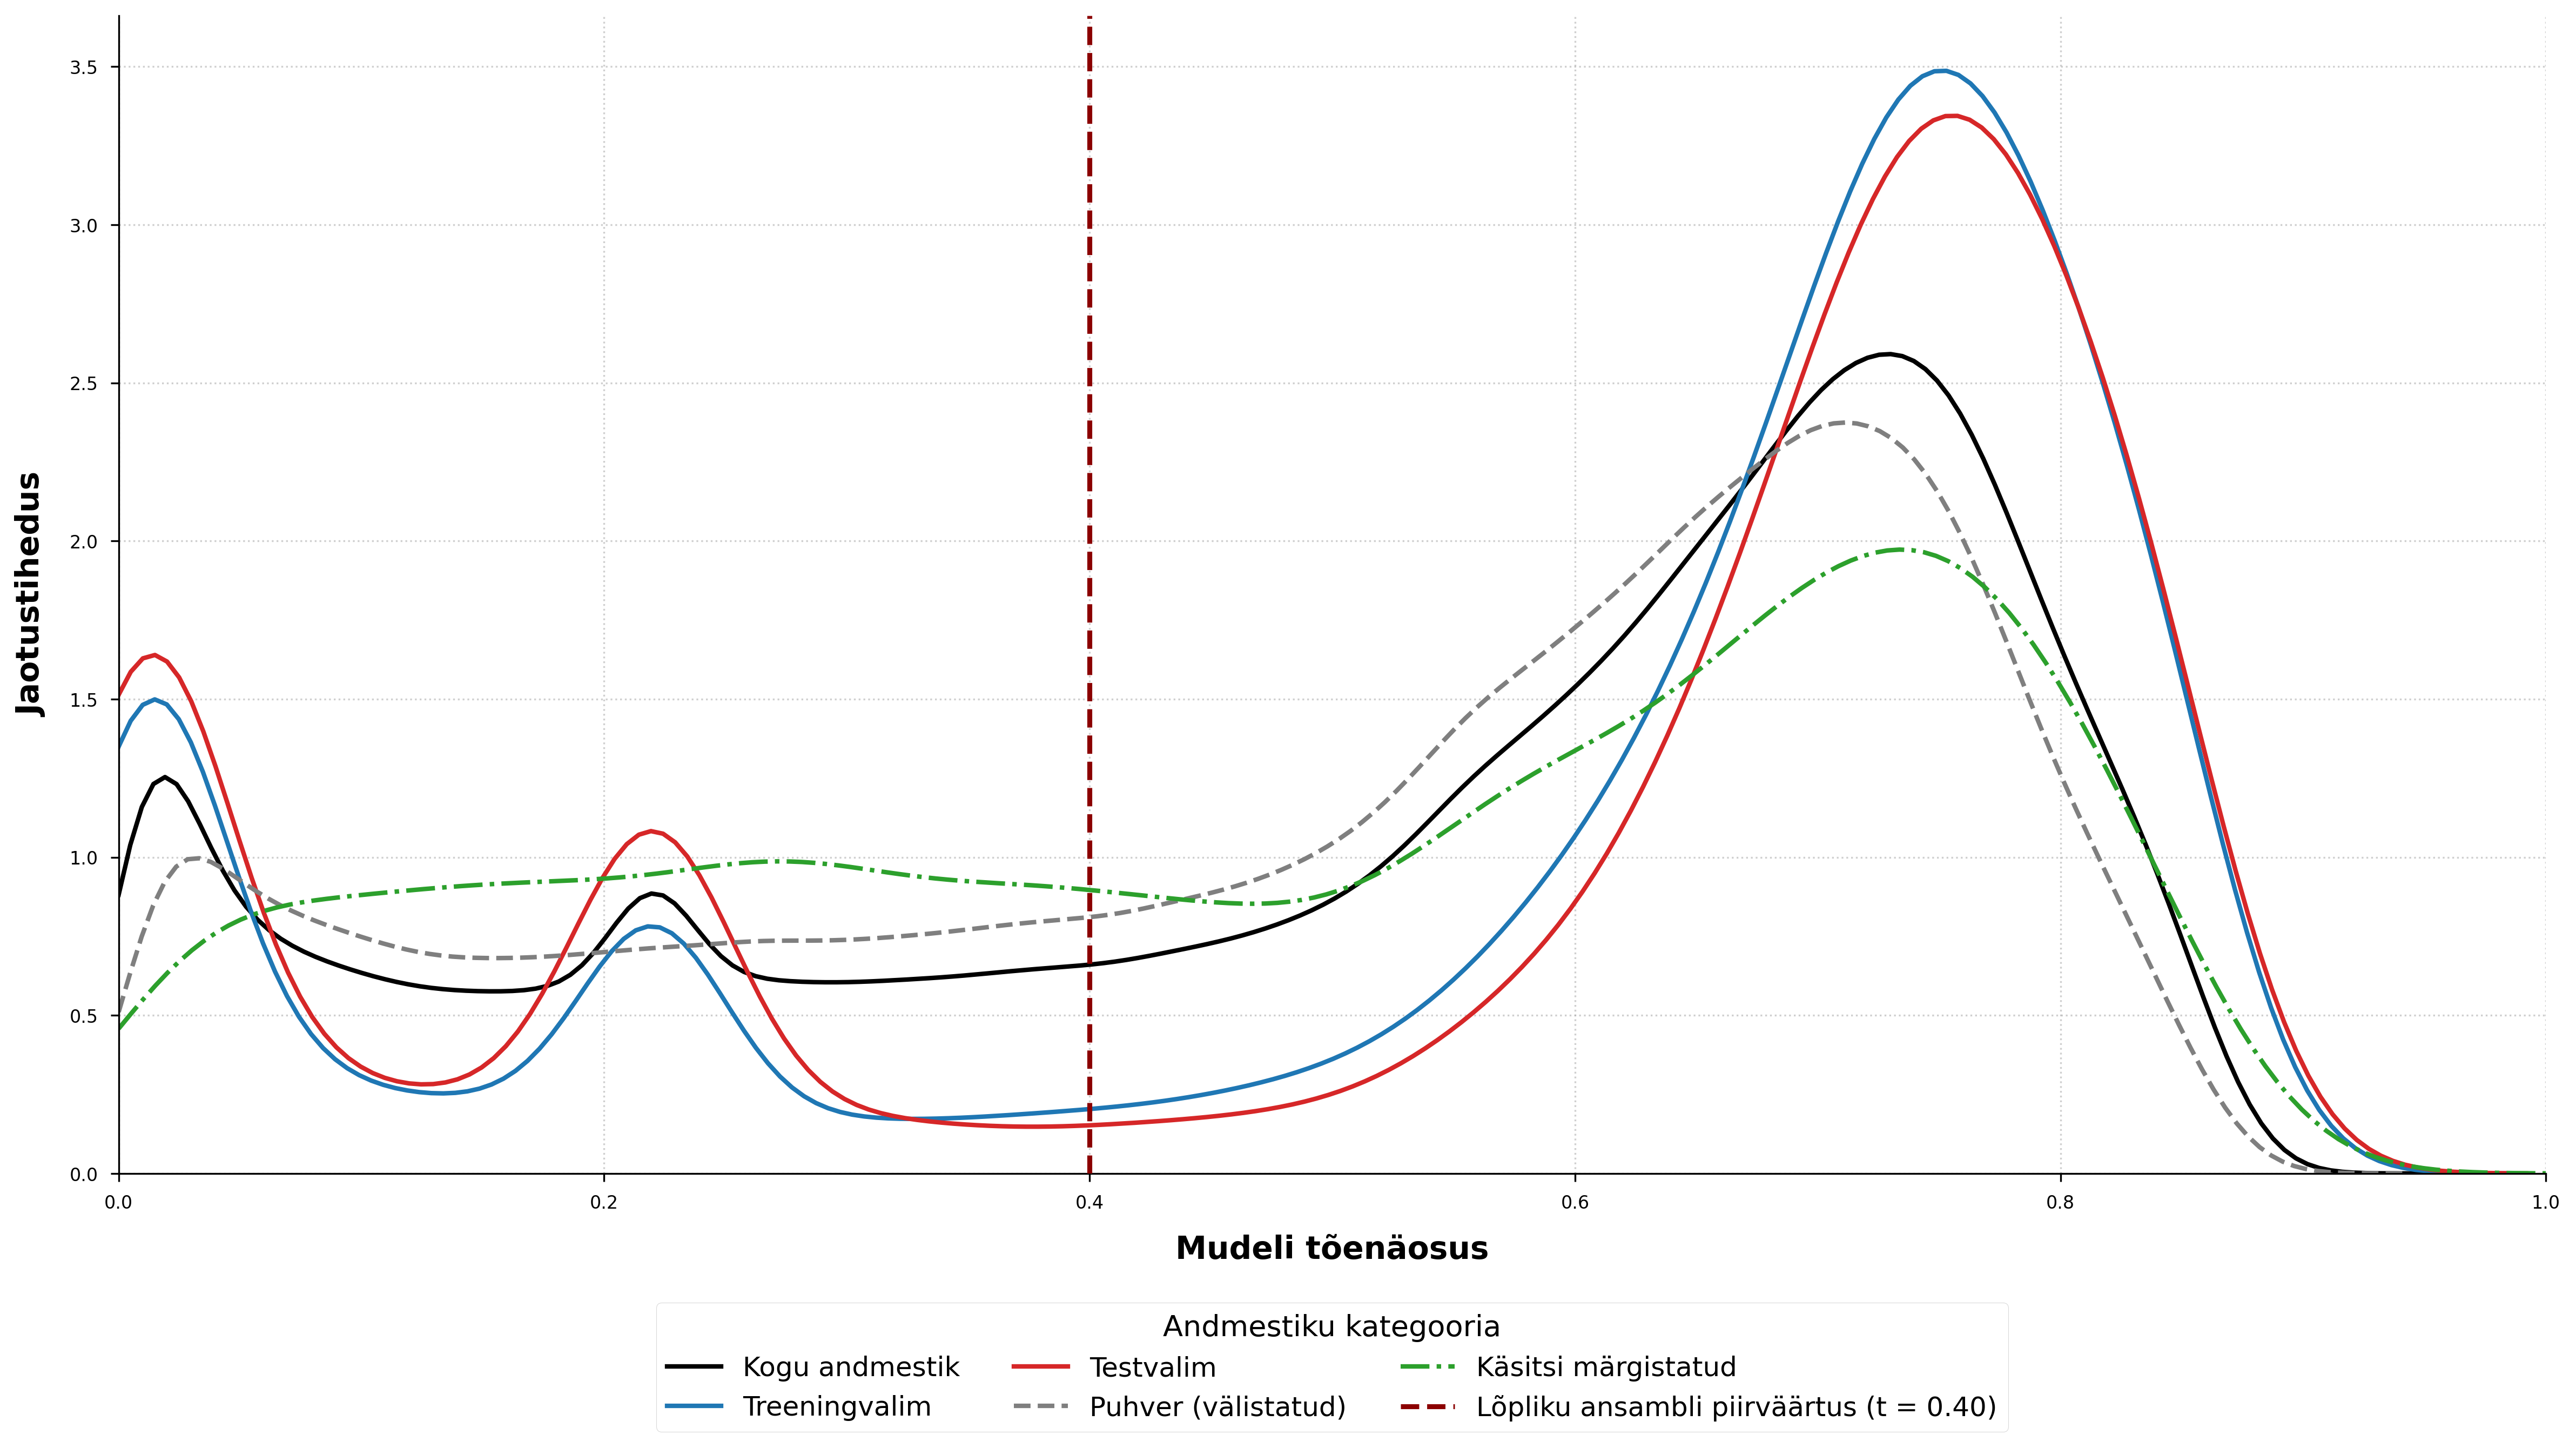
\includegraphics[width=1\linewidth]{estonian/joonised/andmestiku_jaotus.png}
\caption{Klassifitseerimise andmestiku tihedusjaotus mudeli ennustatud tõenäosuse lõikes. Graafik näitab mudeli kindlust (x-telg) erinevates andmejaotustes: kogu korpus, treening-, test- ja väljajäetud puhverala struktuur ning spetsiaalselt käsitsi märgistatud andmepunktide jaotus (mis katab ühtlasemalt ka keskse määramatuse vahemikku).}
\label{fig:andmestiku_jaotus}
\end{figure}

\subsubsection{Ansambli agregeerimismeetodite ja kandidaatide võrdlus}
\label{ansambli-agregeerimise-tulemused}

Pärast aktiivõppega laiendatud märgistusandmestiku moodustamist võrreldi neljanda ansambliliikme ja tõenäosuste agregeerimise alternatiive 5$\times$5 ristvalideerimise raamistikus. Eesmärk oli valida kindel täiendus kolme CNN-Deep-Attn baasmudelile. Võrdlus näitas, et EfficientNet-B2 lisamine täiendas neid kõige paremini. Meetoditest saavutas kaalutud hääletus (ingl \textit{weighted vote}) kõrgeima keskmise F1-skoori ($0{,}9866$), olles logistilise regressiooni virnaansambliga samaväärne, ent tõlgendatavam (Tabel~\ref{tab:ensemble-methods-comparison}).

\begin{table}[h!]
\centering
\caption{Ansambli agregeerimismeetodite võrdlus 5$\times$5 ristvalideerimisel (25 hindamist). Kõik edasised täiustatud meetodid edestavad lihtsat pehmet hääletust statistiliselt olulisel määral.}
\label{tab:ensemble-methods-comparison}
\begin{tabular}{lllcc}
\hline
\textbf{Kandidaat} & \textbf{Meetod} & \textbf{F1 95\% UV} & \textbf{AUC} & \textbf{$p$ vs lihtne} \\
\hline
EfficientNet-B2 & Pehme hääletus           & [0,9804; 0,9843] & 0,9761 & --- \\
EfficientNet-B2 & Pehme h. (häälest.~lävi) & [0,9819; 0,9855] & 0,9761 & 0,0011 ** \\
EfficientNet-B2 & \textbf{Kaalutud hääletus} & \textbf{[0,9849; 0,9883]} & \textbf{0,9810} & $\mathbf{<0{,}0001}$ *** \\
EfficientNet-B2 & Virnaansambel (LR)       & [0,9849; 0,9881] & 0,9810 & $<0{,}0001$ *** \\
EfficientNet-B2 & Virnaansambel (MLP)      & [0,9837; 0,9873] & 0,9802 & $<0{,}0001$ *** \\
\hline
ConvNeXt-tiny   & Pehme hääletus           & [0,9802; 0,9839] & 0,9754 & --- \\
ConvNeXt-tiny   & Virnaansambel (LR)       & [0,9819; 0,9853] & 0,9778 & 0,0002 *** \\
ConvNeXt-tiny   & Virnaansambel (MLP)      & [0,9824; 0,9857] & 0,9772 & 0,0014 ** \\
\hline
ConvNeXt-small  & Pehme hääletus           & [0,9788; 0,9825] & 0,9757 & --- \\
ConvNeXt-small  & Virnaansambel (LR)       & [0,9842; 0,9872] & 0,9789 & $<0{,}0001$ *** \\
ConvNeXt-small  & Kaalutud hääletus        & [0,9839; 0,9870] & 0,9789 & $<0{,}0001$ *** \\
\hline
\end{tabular}
\end{table}

\subsubsection{Lõpliku ansambli jõudlus}
\label{lopliku-ansambli-tulemused}

Lõplik (neljamudeline) ansambel treeniti 67\,290 lekkekontrolliga märgistusel. Testikomplektil ($56\,521$ märgistust) ulatus F1-skoor $0{,}9819$-ni ning ROC AUC väärtus $0{,}9885$-ni. Ansamblipõhine lähenemine aitas eeskätt kaasa raskesti eristatavatel maastikel lokaalse müra tasandamisele.

\begin{figure}[h!]
\centering
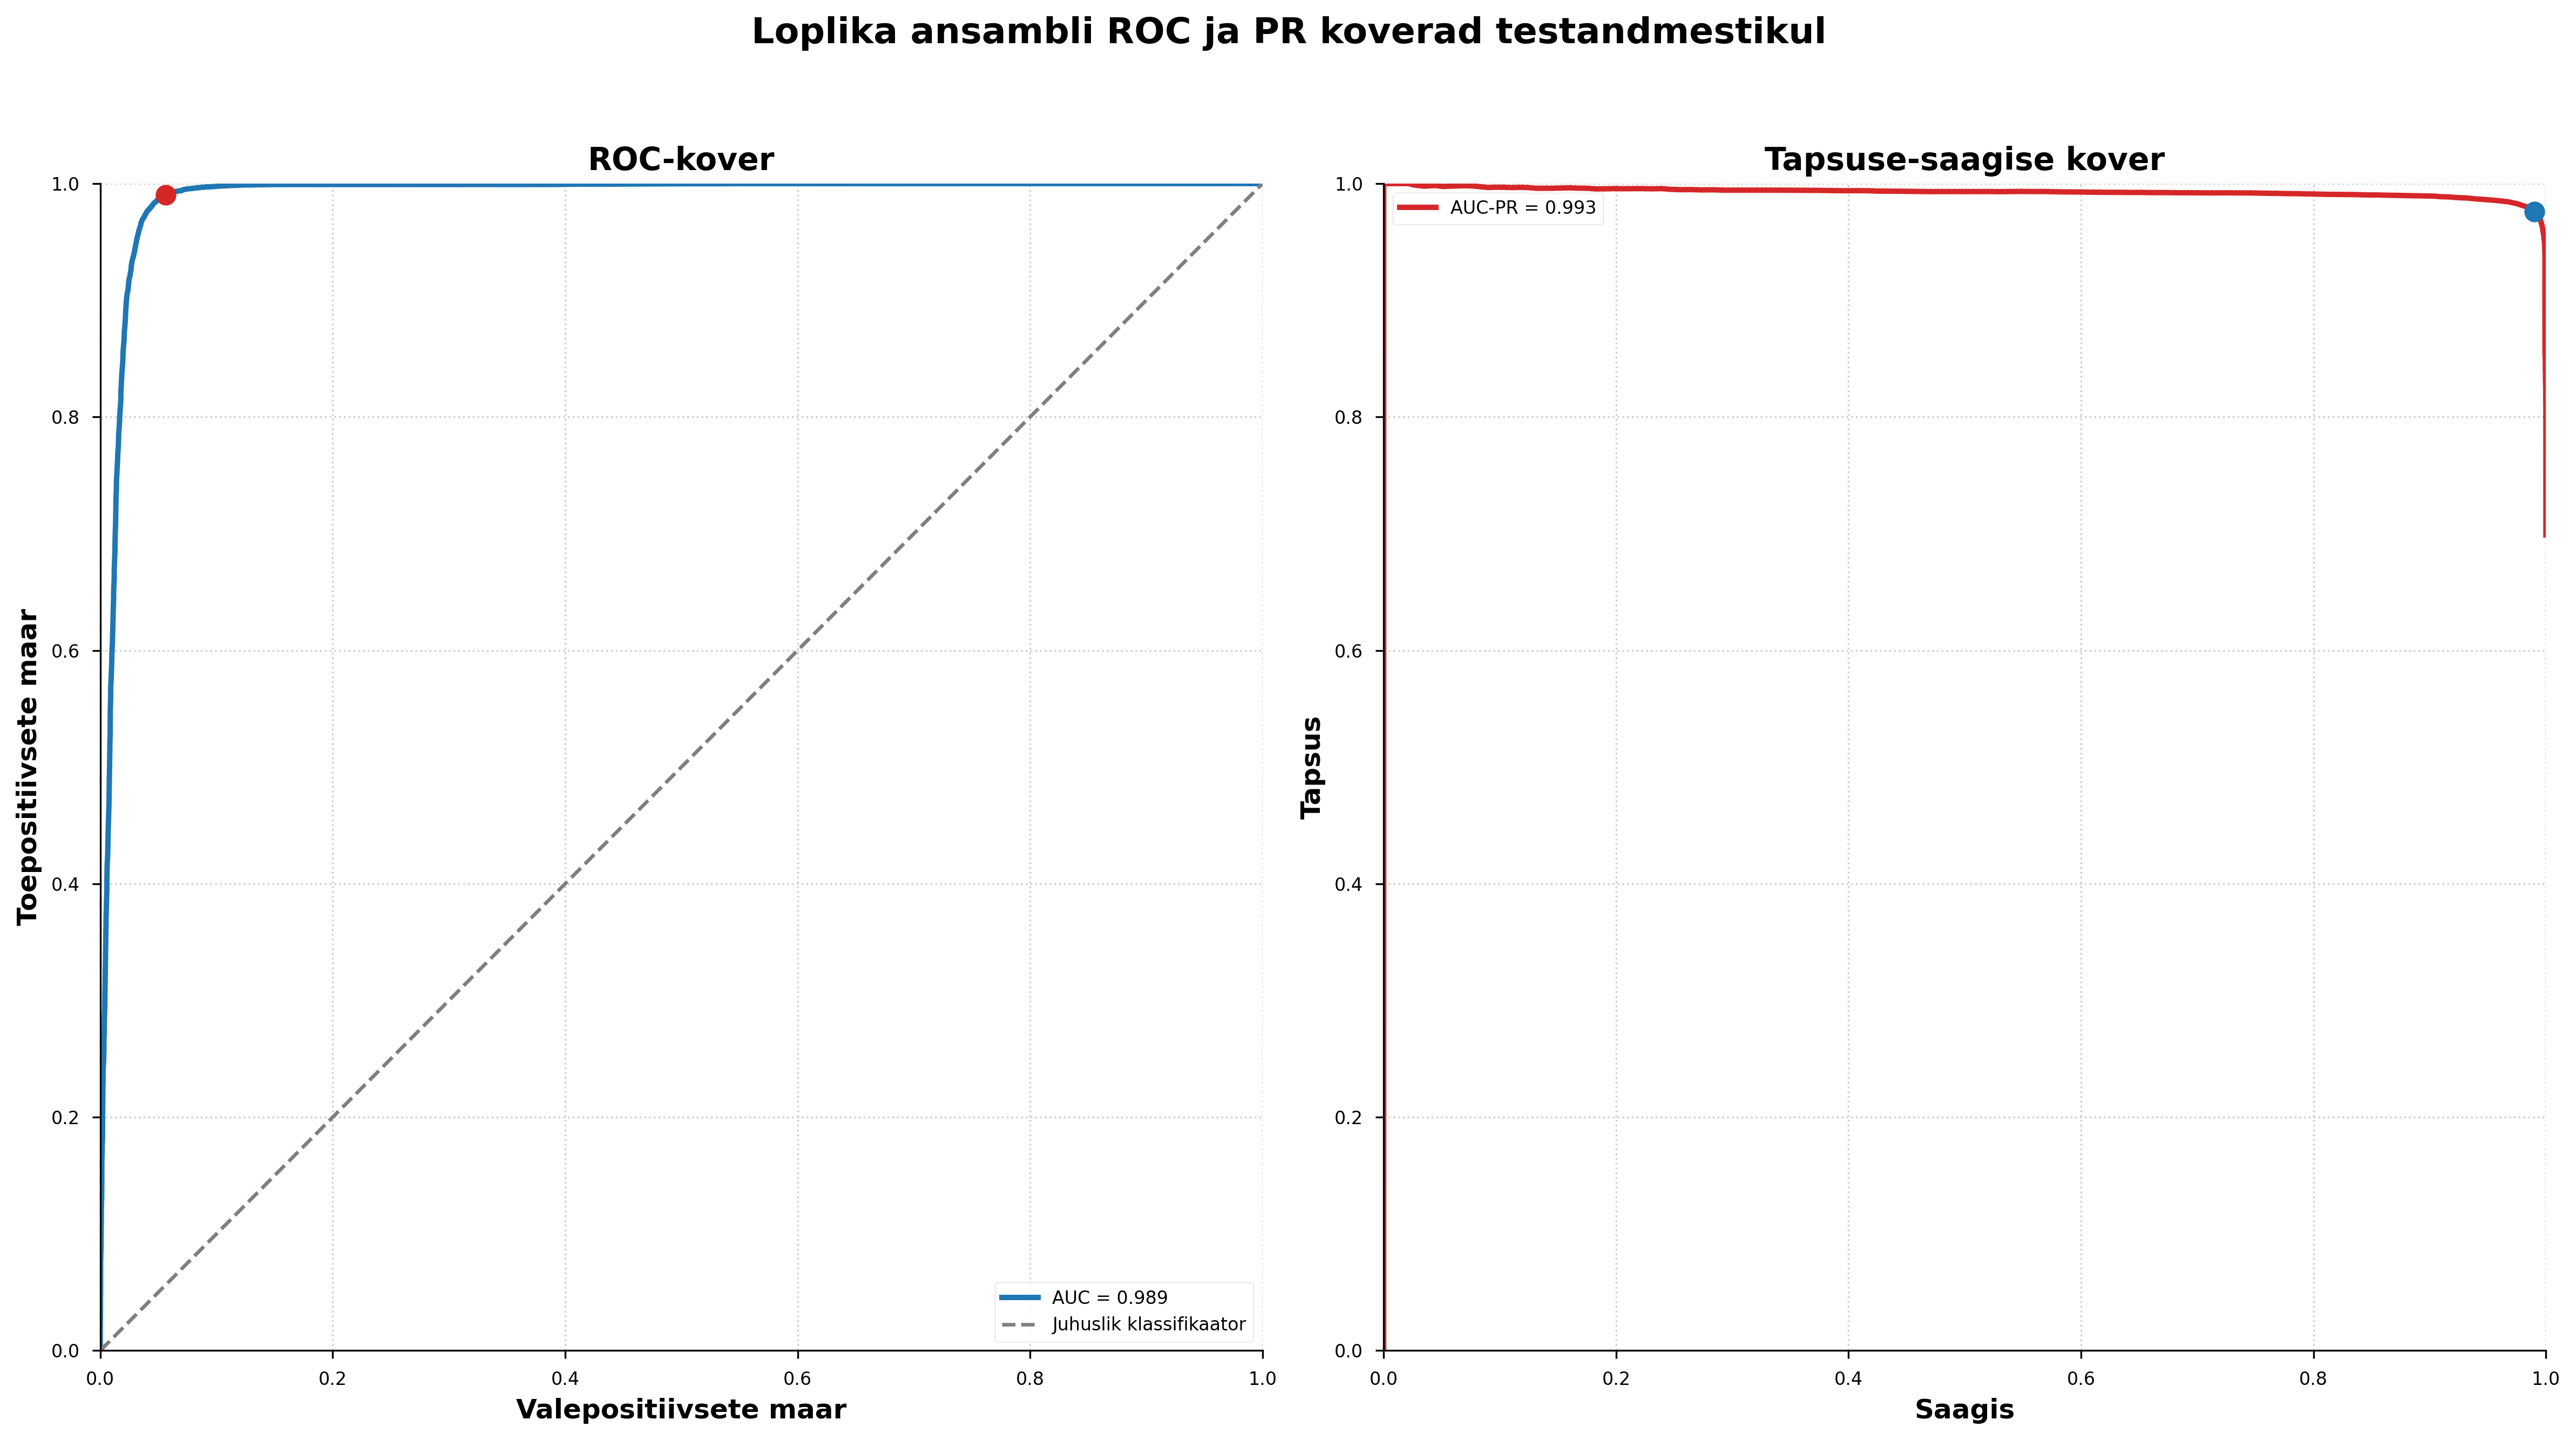
\includegraphics[width=0.95\linewidth]{estonian/joonised/roc_pr_kover_loplik_ansambel.png}
\caption{Mudeli eristusvõimet demonstreerivad ROC ja PR kõverad.}
\label{fig:roc-pr-curve}
\end{figure}

\subsubsection{Taimkatte mudeli variantide võrdlus klassifitseerimises ja segmenteerimises}
\label{chm-variantide-klassifitseerimise-tulemused}

Treeningfaasi esialgsetes eksperimentides vaadeldi mitmeid CHM-i arvutusmudeleid (näiteks erineva kõrgusfiltriga rastersisendid ja mitmekanalilised komposiidid). Lõplikus arenduses ja andmete märgistamise töövoos rakendati 20 cm resolutsiooniga 0--1,31 m kõrguseid filtreerivat ülekünnise väärtuste eemaldamise meetodit.

Segmenteerimismudelite otsinguprotsessis (V6) hinnati süstemaatiliselt viit erinevat CHM-sisendit, et määrata optimaalne sisendandmete esitusviis. Tabelist~\ref{tab:chm_variant_comparison} nähtub, et nelikanalilise composite-variandi (algne + Gaussi silutud + maskeeritud CHM) test-Dice saavutas väärtuse 0,241 ± 0,032, mis ühekanalilisest baasmudelit ületab 13,7\% võrra (0,212 ± 0,026). Sarnane muster ilmnes ka F1-skooris, kus composite saavutas 0,301 ± 0,041 võrreldes baasmudelil 0,260 ± 0,034.

\begin{table}[h]
\centering
\small
\begin{tabular}{lcccc}
\hline
\textbf{CHM-variant} & \textbf{Kanalite arv} & \textbf{Best Dice} & \textbf{Best F1} & \textbf{Suhteline kiirus} \\
\hline
Composite (alg. + gauss + mask) & 4 & 0,241 ± 0,032 & 0,301 ± 0,041 & 1,0× (ref.) \\
Gauss (silutud) & 1 & 0,231 ± 0,028 & 0,285 ± 0,037 & ~1,2× \\
Masked (maskeeritud) & 1 & 0,216 ± 0,023 & 0,265 ± 0,031 & ~1,2× \\
Baseline (algne) & 1 & 0,212 ± 0,026 & 0,260 ± 0,034 & ~1,3× \\
Raw (töötlemata) & 1 & 0,205 ± 0,031 & 0,252 ± 0,040 & ~1,3× \\
\hline
\end{tabular}
\caption{Segmenteerimismudelite (V6) CHM-variantide võrdlus: jõudlus (Dice ja F1) ning suhtelised treenings- ja inferentsiajad. Composite-variant saavutab parima klassifikatsiooni, kuid ühekanaliline baasmudel on märkimisväärselt kiirem.}
\label{tab:chm_variant_comparison}
\end{table}

Klassifitseerimiskatsetes rakendati sarnast loogika. Eksperimendid mitme kanaliga (koondades suhteliskõrguseid ja silutud väärtusi) pakkusid marginaalset täpsuse kasvu (alla 1\% F1 suhtes), kuid suurendasid andmemahtu ja treeningkorduste aega enam kui kolm korda. Tehtud kuluanalüüsist lähtuvalt otsustati klassifitseerimis- ja segmenteerimistöövoos 1-kanalise 20 cm rasteri kasuks, mis pakub tõhusama tasakaalu andmelihtsuse, arvutusresursside ja lõpliku tuvastusvõimekuse vahel.

\subsubsection{Klassifitseerimismudelis esinevate vigade analüüs}
\label{klassifitseerimise-vigade-analüüs}

Vaatamata kõrgele F1-skoorile esines mudeli ennustustes mõningaid iseloomulikke veamustreid. Vead saab valdavalt kategoriseerida lamapuiduga sarnase kujuga objektide väärtuvastamiseks (valepositiivsed) ning tugeva võrastiku/alusmetsa varju jäävate või tugevalt lagunenud lamapuude märkamata jätmiseks (valenegatiivsed).

\paragraph{Valepositiivsed (FP)} Mudel kaldus aeg-ajalt lamapuiduks klassifitseerima vanu kuivenduskraavide kaldavalle, piklikke kivimoodustisi (näiteks vanad aiavaremed) ning teatud juhtudel masinate rööpaid. Neid struktuure iseloomustab lokaalses kõrgusmudelis sirgjooneline anomaalia, mis 20 cm CHM-pikslite puhul võib sarnaneda tüvele.

\paragraph{Valenegatiivsed (FN)} Valenegatiivseid ilmnes enamasti raielankidel, kus tüvi oli hunnikus, pooleksmurdunud või vajunud tugevalt masse. Sellised puud ei kerki 1,3 m CHM kihist selgelt esile ningka  >18 pts/m$^2$ LiDAR andmestik ei taga alati piisavat detailsust maapinnalähedase kuju säilitamiseks.


\paragraph{Käsitsi märgendatud andmestiku tehtud vead.}

Käsitsi märgendatud valimile teostatud täiendav vigade analüüs paljastas, et vastupidiselt kõrgele keskmisele tulemile oli mudel võimeline vigu tegema. Joonisel~\ref{fig:error-case-studies} on esitatud kaks ilustratiivset juhust: (i) Valepostiivne (FP, usaldus 0,9889) -- mudel arvas 128×128 paanil kuuluvat täielikult lamapuitu, kuigikuigi sellel oli ikkagi oli sirge tüvi nähtaval; (ii) Valenegatiivsus (FN, ennustus 0,0249) -- sama kaardilehel olev tegelik lamapuidupaan jäi mudeli tähelepanu all täiesti märkamata, vihjates tugevale vastaste võimaluste osakaalule metsas kasvava võrastiku all. Esimene juhtum süstematiseerib meie jälgitut FP-riske (kraavid, rattarööpad jne.), teine aga selgitab FN-i loomust: andmete ebapiisav hajusus (>18 pts/m² LiDAR) piisavalt hästi kirjeldab peent tüvedome kontuurit, mis on oluline tingimus, et mudel saaks õppida kindlakstegemiseks.

\begin{figure}[h!]
\centering
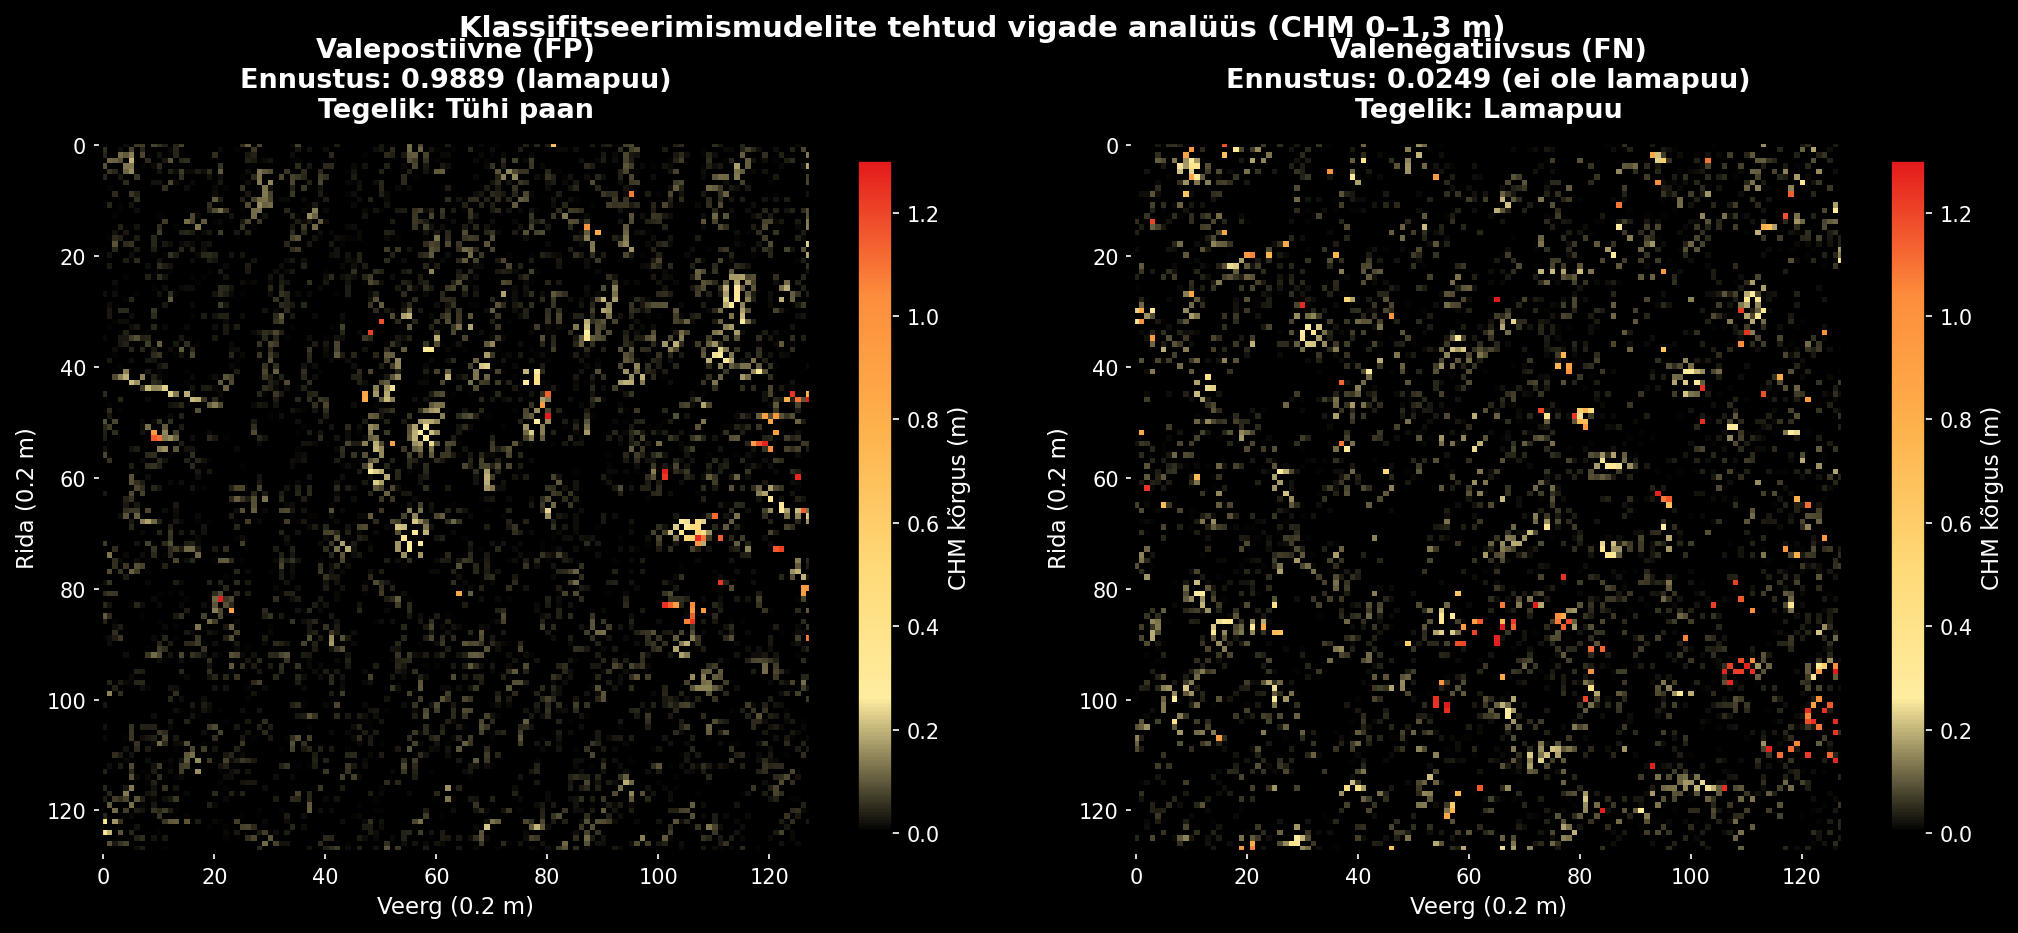
\includegraphics[width=0.95\linewidth]{estonian/joonised/error_cases_comparison.png}
\caption{Klassifitseerimismudelite edenamatust juhtumid käsitsi märgendatud valimis: (vasakul) valepostiivne paan, kus mudel arvas kõrgete usaldusega (98,89\%) lamapuitu, kuid tegelikult oli paan tühi; (paremal) valenegatiivsus, kus tegelik lamapuu pandi mudelile peaaegu nähtamatuks (2,49\% ennustus). Mõlemad juhtumid kaardilehel 465663\_2023\_madal\_chm\_max\_hag\_20cm.tif.}
\label{fig:error-case-studies}
\end{figure}

\paragraph{Aktiivõppiõppe kaksepoolne õppimisprotsess.}

Analüüsitud vigade juhtumid (eriti valepostiivne kõrge usaldusega ja valenegatiivsus madala usaldusega) viitavad tõenäoliselt sellele, et need paanid märgistati käsitsi valesti. Selline olukord demonstreerib aktiivõppet kahepoolselt õppimisprotsessi: mudel ei õpi mitte ainult paranduste kaudu õigete ja valede ennustuste eristamisest, vaid töö autor omakorda õpib kiiremini ja süstemaatilisemalt märgendama edaspidi samasuguseid struktuure. Järjepidevalt paanil 465663 esinevate vastastikuste vigade (kõrge FP ja madal FN samal rasteril) tõttu omandab selle konkreetse maastikutüübi märgendamise mustrid ning vältib edaspidi samade vigade kordamist. Selline pöördteave mudelist on oluline osa aktiivõppega juhitud andmestiku koostamisel ning aitab lõppkokkuvõttes saavutada ühtlast ja kvaliteetset tulemuse.

\subsection{Segmenteerimise tulemused}
\label{segmenteerimise-tulemused}

\paragraph{Kombinatsioonide tähistuste seletus.}

Mudeliotsingu etappides kasutatakse hierarhilist tähistamist \texttt{2X\_\_3Y\_\_4Z\_\_5W\_\_6}, kus iga täht tähistab kindla valiku faasi. Tabel~\ref{tab:seg-notation-legend} koondab kõikide faasidega vastavad tähed ja nende tähendused.

\begin{table}[h!]
\centering
\caption{Segmenteerimismudelite otsingu kombinatsioonide tähistuste seletus (faasid 2--6).}
\label{tab:seg-notation-legend}
\begin{tabular}{ll}
\hline
\textbf{Tähistus} & \textbf{Tähendus} \\
\hline
\multicolumn{2}{l}{\textit{Faas 2: CHM sisendivariant}} \\
\hline
2A & Baseline (20 cm, 0--1,31 m) \\
2B & Raw CHM (töötlemata) \\
2C & Gauss (Gaussi silutud, $\sigma=0,2$) \\
2D & Masked (kaetisega maskeeritud) \\
2E & Composite (komposiitne, mitmekanaliline) \\
\hline
\multicolumn{2}{l}{\textit{Faas 3: Semantiline arhitektuur}} \\
\hline
3B & Unet++ EfficientNet-B0 \\
3C & Unet++ EfficientNet-B2 \\
3E & DeepLabV3+ EfficientNet-B2 \\
\hline
\multicolumn{2}{l}{\textit{Faas 4: Kaofunktsioon}} \\
\hline
4A & DiceFocal \\
4D & Tversky ($\alpha=0{,}5$, $\beta=0{,}5$) \\
4F & Tversky ($\alpha=0{,}7$, $\beta=0{,}3$) \\
4H & Tversky + clDice ($\lambda=0{,}3$) \\
\hline
\multicolumn{2}{l}{\textit{Faas 5: Andmerikastamine ja regulariseerimine}} \\
\hline
5A & Andmerikastamist ei kasutatud \\
5D & Täielik augment + pehmed sihtväärtused + SWA (on) \\
5E & Täielik augment + pehmed sihtväärtused, SWA (välja) \\
\hline
\multicolumn{2}{l}{\textit{Faas 6}} \\
\hline
6 & Lõpphindamine eraldiseisvatel testplokkidel (42 paani) \\
\hline
\end{tabular}
\end{table}

\subsubsection{Segmenteerimisandmestiku ja valideerimise metoodika}
\label{segmenteerimise-andmestik-metoodika}

Segmenteerimiskatse viidi läbi välistamisanalüüsi metoodika alusel, kus igast otsingu faasist pääses edasi kaks parimat lahendust. Mudelite valik (faasid 2--5) tehti ainult ristvalideerimise põhjal ning eraldiseisvaid testplokke kasutati üksnes lõpphinnanguks faasis 6. Selline protseduur väldib testileket ning hoiab mudeli valiku ja lõpphinnangu rangelt lahus.

Kasutati ruumilist CVv5 jaotust: kogu ala jagati mittekattuvateks 256$\times$256 paanideks, paanid agregeeriti 3$\times$3 plokkideks, millest ligikaudu 20\% eraldati testiks. Iga CHM-variandi puhul oli paane kokku 202, neist 42 kuulusid eraldiseisvasse testikomplekti (34 positiivset). Mudelivalikuks jäid 160 paani, mis jaotati kolme ristvalideerimise osale (0, 1, 2). Lõppfaasis treeniti mudelid kõigil mitte-test plokkidel ja hinnati üks kord eraldiseisvatel testplokkidel.

\begin{table}[h!]
\centering
\caption{CVv5 andmejaotuse kokkuvõte segmenteerimiskatsetes (logi preflight-statistika). Positiivsete all mõeldakse paane, milles esineb vähemalt üks lamapuidu piksel.}
\label{tab:seg-cvv5-split}
\begin{tabular}{llll}
\hline
\textbf{Jaotus} & \textbf{Paanide arv} & \textbf{Positiivseid} & \textbf{Kommentaar} \\
\hline
Kokku & 202 & --- & ühe CHM-variandi paanid \\
Eraldiseisev test & 42 & 34 & kasutati ainult faasis 6 \\
Treening+valik kokku & 160 & --- & kasutati faasides 2--5 \\
Osa 0 (val) & 54 & 36 & train 106, suhe 1,96 \\
Osa 1 (val) & 69 & 49 & train 91, suhe 1,32 \\
Osa 2 (val) & 37 & 31 & train 123, suhe 3,32 \\
\hline
\end{tabular}
\end{table}

Valikukriteerium kinnitati enne jooksu: primaarne mõõdik oli \texttt{val\_cldice}; viigimurdmine toimus järjekorras \texttt{mean(val\_cldice)} $\rightarrow$ \texttt{mean(val\_f1)} $\rightarrow$ väiksem \texttt{std(val\_cldice)}. Lisaks rakendati konservatiivset kandidaatide kärpimist arvutusaja vähendamiseks (faas 3: 3B/3C/3E; faas 4: 4A/4D/4F/4H; faas 5: 5A/5D/5E), mis säilitas varasemates katsetes kõige konkurentsivõimelisema otsinguruumi.

\subsubsection{Segmenteerimismudelite otsing ja parameetrite võrdlus}
\label{segmenteerimise-mudeli-otsing}

\paragraph{Testitud arhitektuurid ja sisendvariandid.}

Faasis 2 hinnati viit CHM-sisendit (2A--2E), hoides ülejäänud seadistuse fikseerituna (Unet++ EfficientNet-B2, Tversky $\alpha{=}0{,}6$, $\beta{=}0{,}4$, \textit{clDice}-komponent $\lambda{=}0{,}3$). Tabel~\ref{tab:seg-phase2} näitab, et parimad keskmised \texttt{val\_cldice} väärtused saadi \texttt{composite} ja \texttt{baseline} sisendiga. \texttt{masked} variant jäi selgelt nõrgemaks.

\begin{table}[h!]
\centering
\caption{Faas 2 (CHM variandid): tulemused mõõdikul \texttt{val\_cldice} (koondades kolm osa keskmiseks).}
\label{tab:seg-phase2}
\begin{tabular}{llllll}
\hline
\textbf{Koht} & \textbf{Tingimus} & \textbf{CHM} & \textbf{Mean} & \textbf{SD} & \textbf{Osad (0/1/2)} \\
\hline
1 & 2E & composite & 0,2311 & 0,0476 & 0,2091 / 0,1869 / 0,2972 \\
2 & 2A & baseline  & 0,2206 & 0,0482 & 0,1991 / 0,1754 / 0,2873 \\
3 & 2C & gauss     & 0,2161 & 0,0385 & 0,2022 / 0,1774 / 0,2687 \\
4 & 2B & raw       & 0,2138 & 0,0417 & 0,1924 / 0,1769 / 0,2721 \\
5 & 2D & masked    & 0,1185 & 0,0204 & 0,1046 / 0,1036 / 0,1473 \\
\hline
\end{tabular}
\end{table}

Faasis 3 võrreldi kahte edasi liikunud CHM-kandidaati kolme arhitektuuriga (Unet++B0, Unet++B2, DeepLabV3+B2; kokku 6 kombinatsiooni). Parima tulemuse andis \texttt{2E\_\_3B} (Unet++B0 + composite), mis ületas teist kohta \texttt{2A\_\_3C} marginaalselt, kuid stabiilsemalt (madalam hajuvus kui mitmel alternatiivil).

\begin{table}[h!]
\centering
\caption{Faas 3 (arhitektuur + CHM): \texttt{val\_cldice} järjestus.}
\label{tab:seg-phase3}
\begin{tabular}{llllll}
\hline
\textbf{Koht} & \textbf{Kombinatsioon} & \textbf{Arhitektuur} & \textbf{Mean} & \textbf{SD} & \textbf{Osad (0/1/2)} \\
\hline
1 & 2E\_\_3B & Unet++ EffB0    & 0,2645 & 0,0482 & 0,2410 / 0,2209 / 0,3317 \\
2 & 2A\_\_3C & Unet++ EffB2    & 0,2277 & 0,0714 & 0,1782 / 0,1763 / 0,3286 \\
3 & 2E\_\_3E & DeepLabV3+ EffB2& 0,2224 & 0,0437 & 0,1952 / 0,1880 / 0,2841 \\
4 & 2A\_\_3B & Unet++ EffB0    & 0,2221 & 0,0515 & 0,1960 / 0,1763 / 0,2940 \\
5 & 2A\_\_3E & DeepLabV3+ EffB2& 0,2146 & 0,0512 & 0,1873 / 0,1702 / 0,2862 \\
6 & 2E\_\_3C & Unet++ EffB2    & 0,2131 & 0,0358 & 0,1851 / 0,1905 / 0,2636 \\
\hline
\end{tabular}
\end{table}

\paragraph{Kaofunktsioonid ja andmerikastamised.}

Faasis 4 testiti nelja kaofunktsiooni seadistust mõlemal faasi-3 võitjal (kokku 8 seadistust). Tabel~\ref{tab:seg-phase4} järgi osutusid tugevaimaks kaks \texttt{2E\_\_3B} haru: \texttt{4H} (Tversky + \textit{clDice}) ja \texttt{4A} (DiceFocal). See näitab, et kaofunktsiooni mõju sõltus oluliselt eelnevast arhitektuuri- ja sisendivalikust (koosmõju), mitte ainult üksikust kaotüübist.

\begin{table}[h!]
\centering
\caption{Faas 4 (kaofunktsioonid): \texttt{val\_cldice} tulemused.}
\label{tab:seg-phase4}
\begin{tabular}{llllll}
\hline
\textbf{Koht} & \textbf{Kombinatsioon} & \textbf{Kaofunktsioon} & \textbf{Mean} & \textbf{SD} & \textbf{Osad (0/1/2)} \\
\hline
1 & 2E\_\_3B\_\_4H & Tversky + clDice & 0,2551 & 0,0434 & 0,2221 / 0,2268 / 0,3164 \\
2 & 2E\_\_3B\_\_4A & DiceFocal        & 0,2442 & 0,0448 & 0,2288 / 0,1987 / 0,3051 \\
3 & 2E\_\_3B\_\_4F & Tversky (0,7/0,3)& 0,2367 & 0,0615 & 0,2282 / 0,1658 / 0,3159 \\
4 & 2A\_\_3C\_\_4H & Tversky + clDice & 0,2194 & 0,0324 & 0,2328 / 0,1748 / 0,2507 \\
5 & 2A\_\_3C\_\_4A & DiceFocal        & 0,2002 & 0,0427 & 0,1804 / 0,1608 / 0,2595 \\
6 & 2E\_\_3B\_\_4D & Tversky (0,5/0,5)& 0,1839 & 0,0259 & 0,1643 / 0,1668 / 0,2205 \\
7 & 2A\_\_3C\_\_4D & Tversky (0,5/0,5)& 0,1774 & 0,0130 & 0,1695 / 0,1669 / 0,1957 \\
8 & 2A\_\_3C\_\_4F & Tversky (0,7/0,3)& 0,1633 & 0,0192 & 0,1548 / 0,1452 / 0,1899 \\
\hline
\end{tabular}
\end{table}

Faasis 5 hinnati andmerikastamise/regulariseerimise seadistusi kahel parimaks osutunud kaofunktsiooni seadistusel (kokku 6 seadistust). Tulemused (Tabel~\ref{tab:seg-phase5}) näitavad järjepidevalt, et \texttt{5E} (täielik andmerikastamine + pehmed sihtväärtused, SWA välja lülitatud) andis mõlemas harus kõige tugevama \texttt{val\_cldice}. Teise olulise tähelepanekuna olid mõlemad \texttt{5D} variandid (pehmed sihtväärtused + SWA) selgelt nõrgimad.

\begin{table}[h!]
\centering
\caption{Faas 5 (andmerikastamine/regulariseerimine): \texttt{val\_cldice} tulemused.}
\label{tab:seg-phase5}
\begin{tabular}{llllll}
\hline
\textbf{Koht} & \textbf{Kombinatsioon} & \textbf{Seadistus} & \textbf{Mean} & \textbf{SD} & \textbf{Osad (0/1/2)} \\
\hline
1 & 2E\_\_3B\_\_4H\_\_5E & full+soft, SWA off & 0,3270 & 0,0554 & 0,2876 / 0,2879 / 0,4053 \\
2 & 2E\_\_3B\_\_4A\_\_5E & full+soft, SWA off & 0,3101 & 0,0600 & 0,2650 / 0,2705 / 0,3949 \\
3 & 2E\_\_3B\_\_4H\_\_5A & no aug             & 0,2980 & 0,0516 & 0,2862 / 0,2415 / 0,3662 \\
4 & 2E\_\_3B\_\_4A\_\_5A & no aug             & 0,2765 & 0,0480 & 0,2653 / 0,2240 / 0,3400 \\
5 & 2E\_\_3B\_\_4H\_\_5D & full+soft+SWA      & 0,2222 & 0,0298 & 0,2254 / 0,1841 / 0,2570 \\
6 & 2E\_\_3B\_\_4A\_\_5D & full+soft+SWA      & 0,2005 & 0,0271 & 0,2041 / 0,1658 / 0,2318 \\
\hline
\end{tabular}
\end{table}

\begin{figure}[h!]
\centering
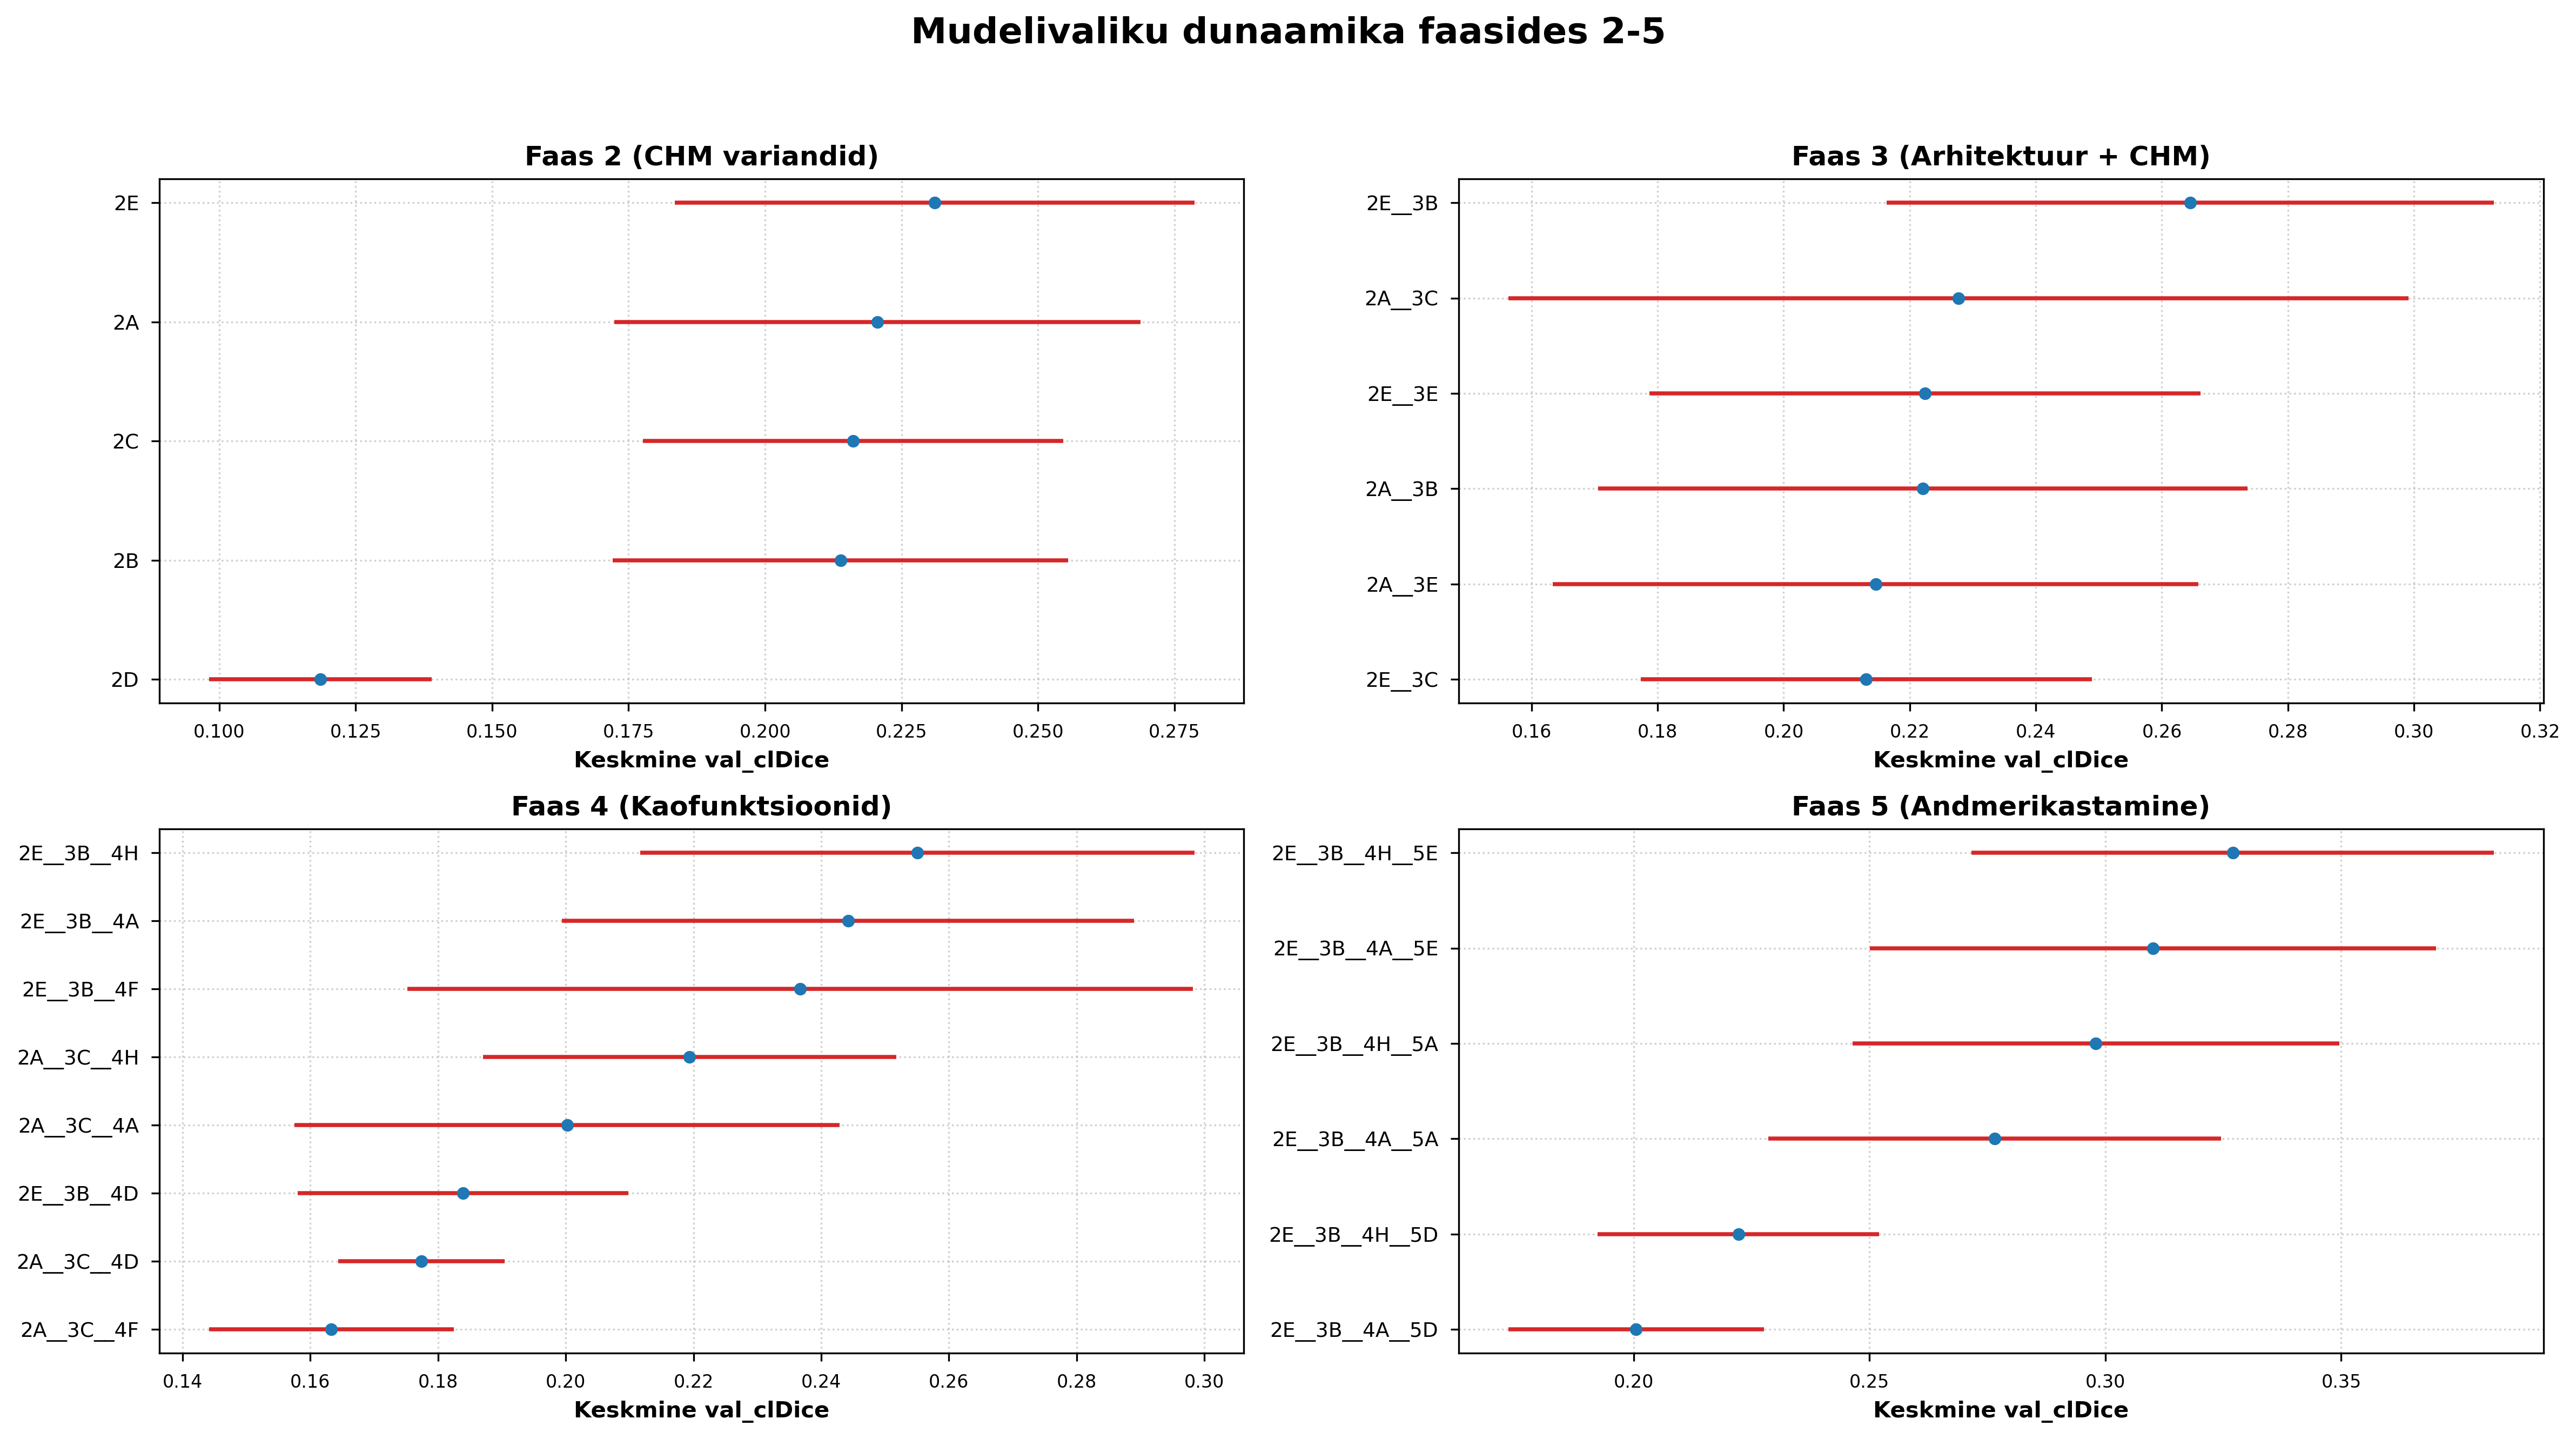
\includegraphics[width=0.95\linewidth]{estonian/joonised/seg_faaside_paremusjarjestus.png}
\caption{Mudelivaliku dünaamika faasides 2--5 ja kandidaatidevahelised erinevused.}
\label{fig:seg-phase-ranking}
\end{figure}

\subsubsection{Lõpliku segmenteerimismudelite jõudlus}
\label{segmenteerimise-lopliku-joudlus}

\paragraph{Parim mudeli seadistus ja testvalimi tulemused.}

Pärast faasi 5 võitjate kinnitamist viidi faasis 6 läbi üksik lõpphindamine eraldiseisval testvalimil (ingl \textit{held-out test}) kolmele eelnevalt määratud mudelile: kaks parimaks osutunud kombinatsiooni ja eelnev standardseadistus (\texttt{2A\_\_3C\_\_4H\_\_5D}). Tabel~\ref{tab:seg-final-test} koondab lõppnäitajad.

\begin{table}[h!]
\centering
\caption{Eraldiseisva testikomplekti tulemused faasis 6 (paremusjärjestus \texttt{test\_f1} järgi).}
\label{tab:seg-final-test}
\begin{tabular}{llllllll}
\hline
\textbf{Mudel} & \textbf{F1} & \textbf{clDice} & \textbf{IoU} & \textbf{Täpsus} & \textbf{Tagasik.} & \textbf{Lävi} & \textbf{Komponendid} \\
\hline
2E\_\_3B\_\_4H\_\_5E\_\_6 & 0,5750 & 0,4173 & 0,4035 & 0,5832 & 0,5671 & 0,50 & 674 \\
2E\_\_3B\_\_4A\_\_5E\_\_6 & 0,5490 & 0,4031 & 0,3784 & 0,5290 & 0,5707 & 0,30 & 1076 \\
2A\_\_3C\_\_4H\_\_5D\_\_6 & 0,4881 & 0,3490 & 0,3229 & 0,4602 & 0,5197 & 0,50 & 1348 \\
\hline
\end{tabular}
\end{table}

Parimaks osutus \texttt{2E\_\_3B\_\_4H\_\_5E\_\_6}, mille test-F1 oli 0,5750 ja test-\textit{clDice} 0,4173. Võrreldes eelneva standardseadistusega paranesid F1 (+0,0869; +17,8\%), \textit{clDice} (+0,0684; +19,6\%) ja IoU (+0,0806; +25,0\%). Samas oli ka parimal mudelil piirjoonte kvaliteedi mõõdik (\textit{boundary IoU}) madal (0,0570), mis viitab, et objektide globaalne tabamine paranes rohkem kui täpne kontuuripõhine kuju taastamine.

\begin{figure}[h!]
\centering
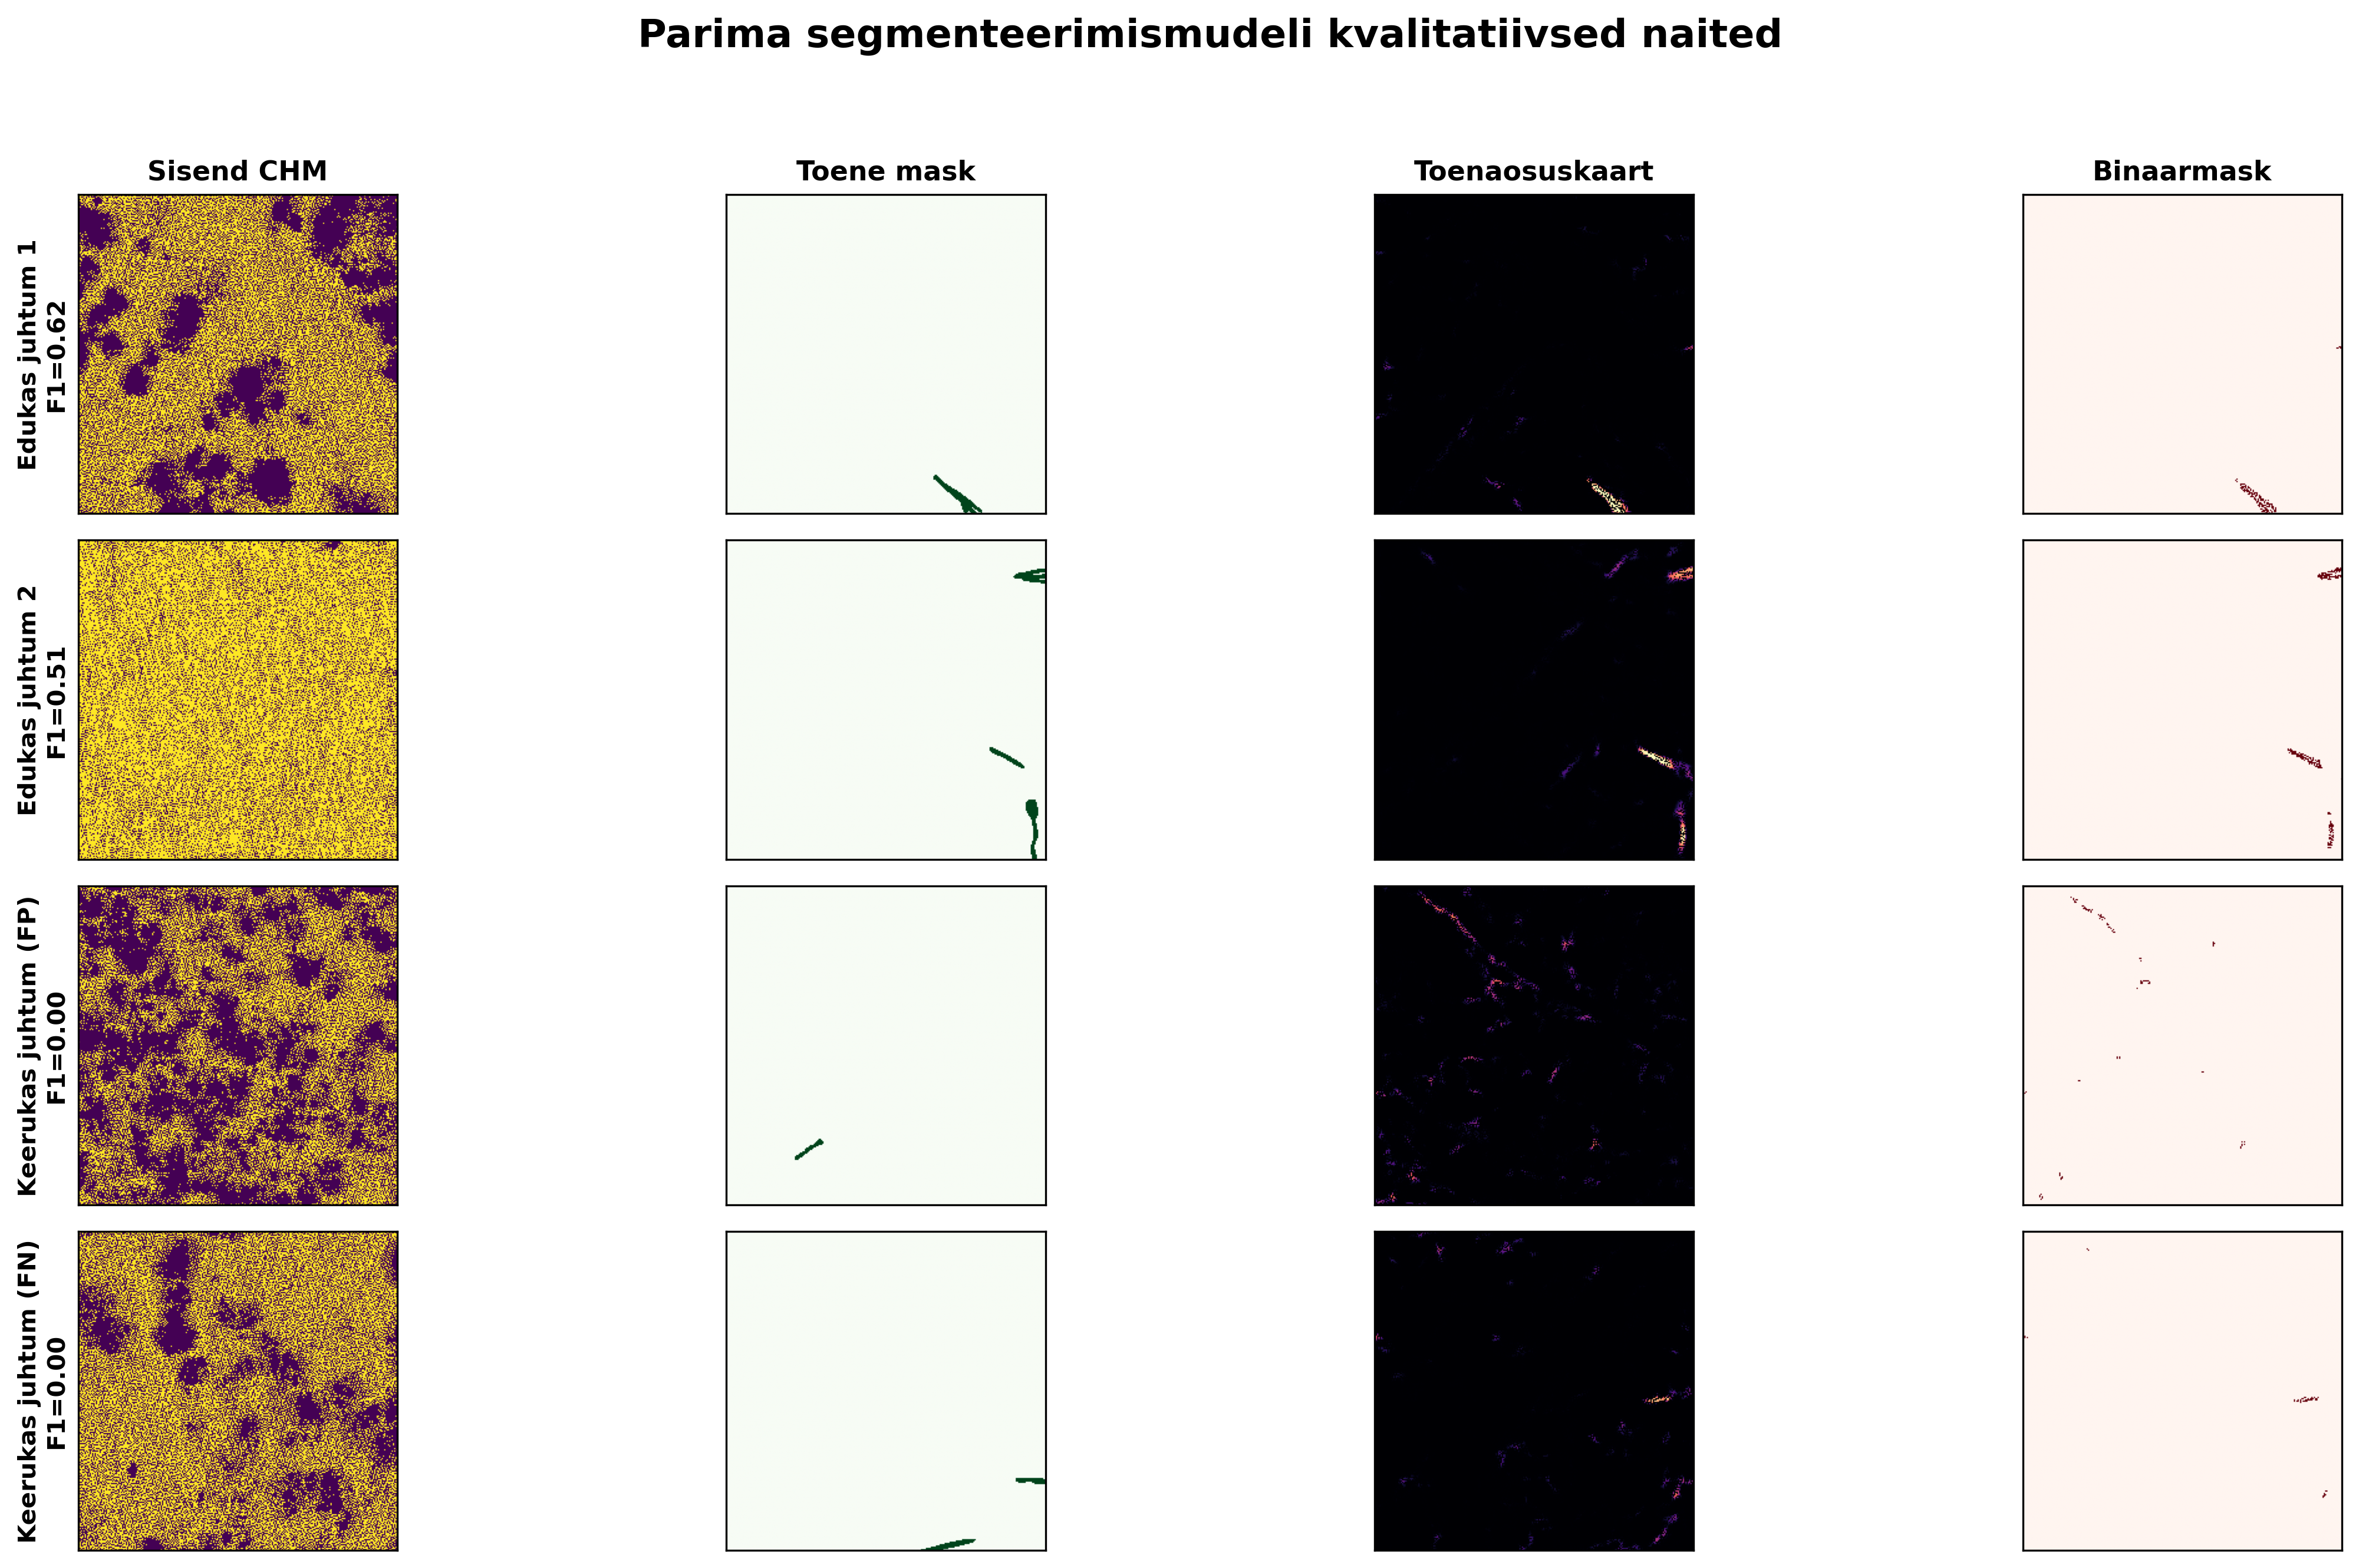
\includegraphics[width=0.95\linewidth]{estonian/joonised/seg_parim_kvalitatiivne.png}
\caption{Parima mudeli kvalitatiivsed tulemused eraldiseisvatel testplokkidel.}
\label{fig:seg-best-qualitative}
\end{figure}

\paragraph{Võrdlus klassifitseerimise baaslähenemisega.}

Käesolevas logipõhises välistamisanalüüsis ei hinnatud eraldi klassifitseerimisest tuletatud pikslimaski (s.t. otsene pikslitasandi (ingl \textit{pixel-level}) võrdlus klassifitseerimisahelaga puudub). Seetõttu on kvantitatiivne võrdlus selles alapeatükis piiratud kolme segmenteerimisseadistuse omavahelise võrdlusega (kaks parimaks osutunud kandidaati + varasemalt leitud parima mudeli ahel).

Metoodika, kus igast faasist pääses edasi kaks parimat lahendust, leidis varasemast lahendusest oluliselt tugevama segmenteerimislahenduse. Otsene väide ``segmenteerimine vs klassifitseerimine'' eeldab siiski täiendavat kontrollkatset, kus samal eraldiseisval testialal mõõdetakse paralleelselt ka klassifitseerimispõhise maski \textit{clDice}, IoU ja F1.

\subsubsection{Generaliseerimuse valideerimise tulemused}
\label{segmenteerimise-generaliseerimine}

Generaliseerimisvõime hindamiseks oli oluline, et testplokid olid mudelivalikust täielikult eraldatud. Faaside 2--5 valik tehti ainult \texttt{val\_cldice} põhjal ristvalideerimise osades ning alles pärast võitjate kinnitamist hinnati mudeleid testil. Seega peegeldavad tabeli~\ref{tab:seg-final-test} tulemused realistlikku üldistusvõimet, mitte valideerimisel ületreenimist.

Samas ilmnes märgatav ruumiline heterogeensus: peaaegu kõigis faasides andis osa 2 oluliselt kõrgema \texttt{val\_cldice} kui osad 0 ja 1. See viitab, et osad plokid on struktuurilt lihtsamad (või parema signaali-müra suhtega) kui teised. Selline muster ei invalideeri tulemust, kuid tähendab, et lõpphinnangu kõrval tuleb raporteerida ka osadevaheline hajuvus (mida tehti kõikides faasitabelites SD kaudu).

Lisaks näitab komponentide arv testis (674 vs 222 tõelist objekti ka parima mudeli puhul), et mudel kipub jätkuvalt üle-segmenteerima peenstruktuure. Seetõttu on järgmise arendussammu kriitiline suund piiri- ja objektitaseme regulariseerimine (nt komponentide järeltöötlus, ühenduvuspõhised piirangud, boundary-loss), mitte üksnes globaalse F1 suurendamine.

\begin{figure}[h!]
\centering
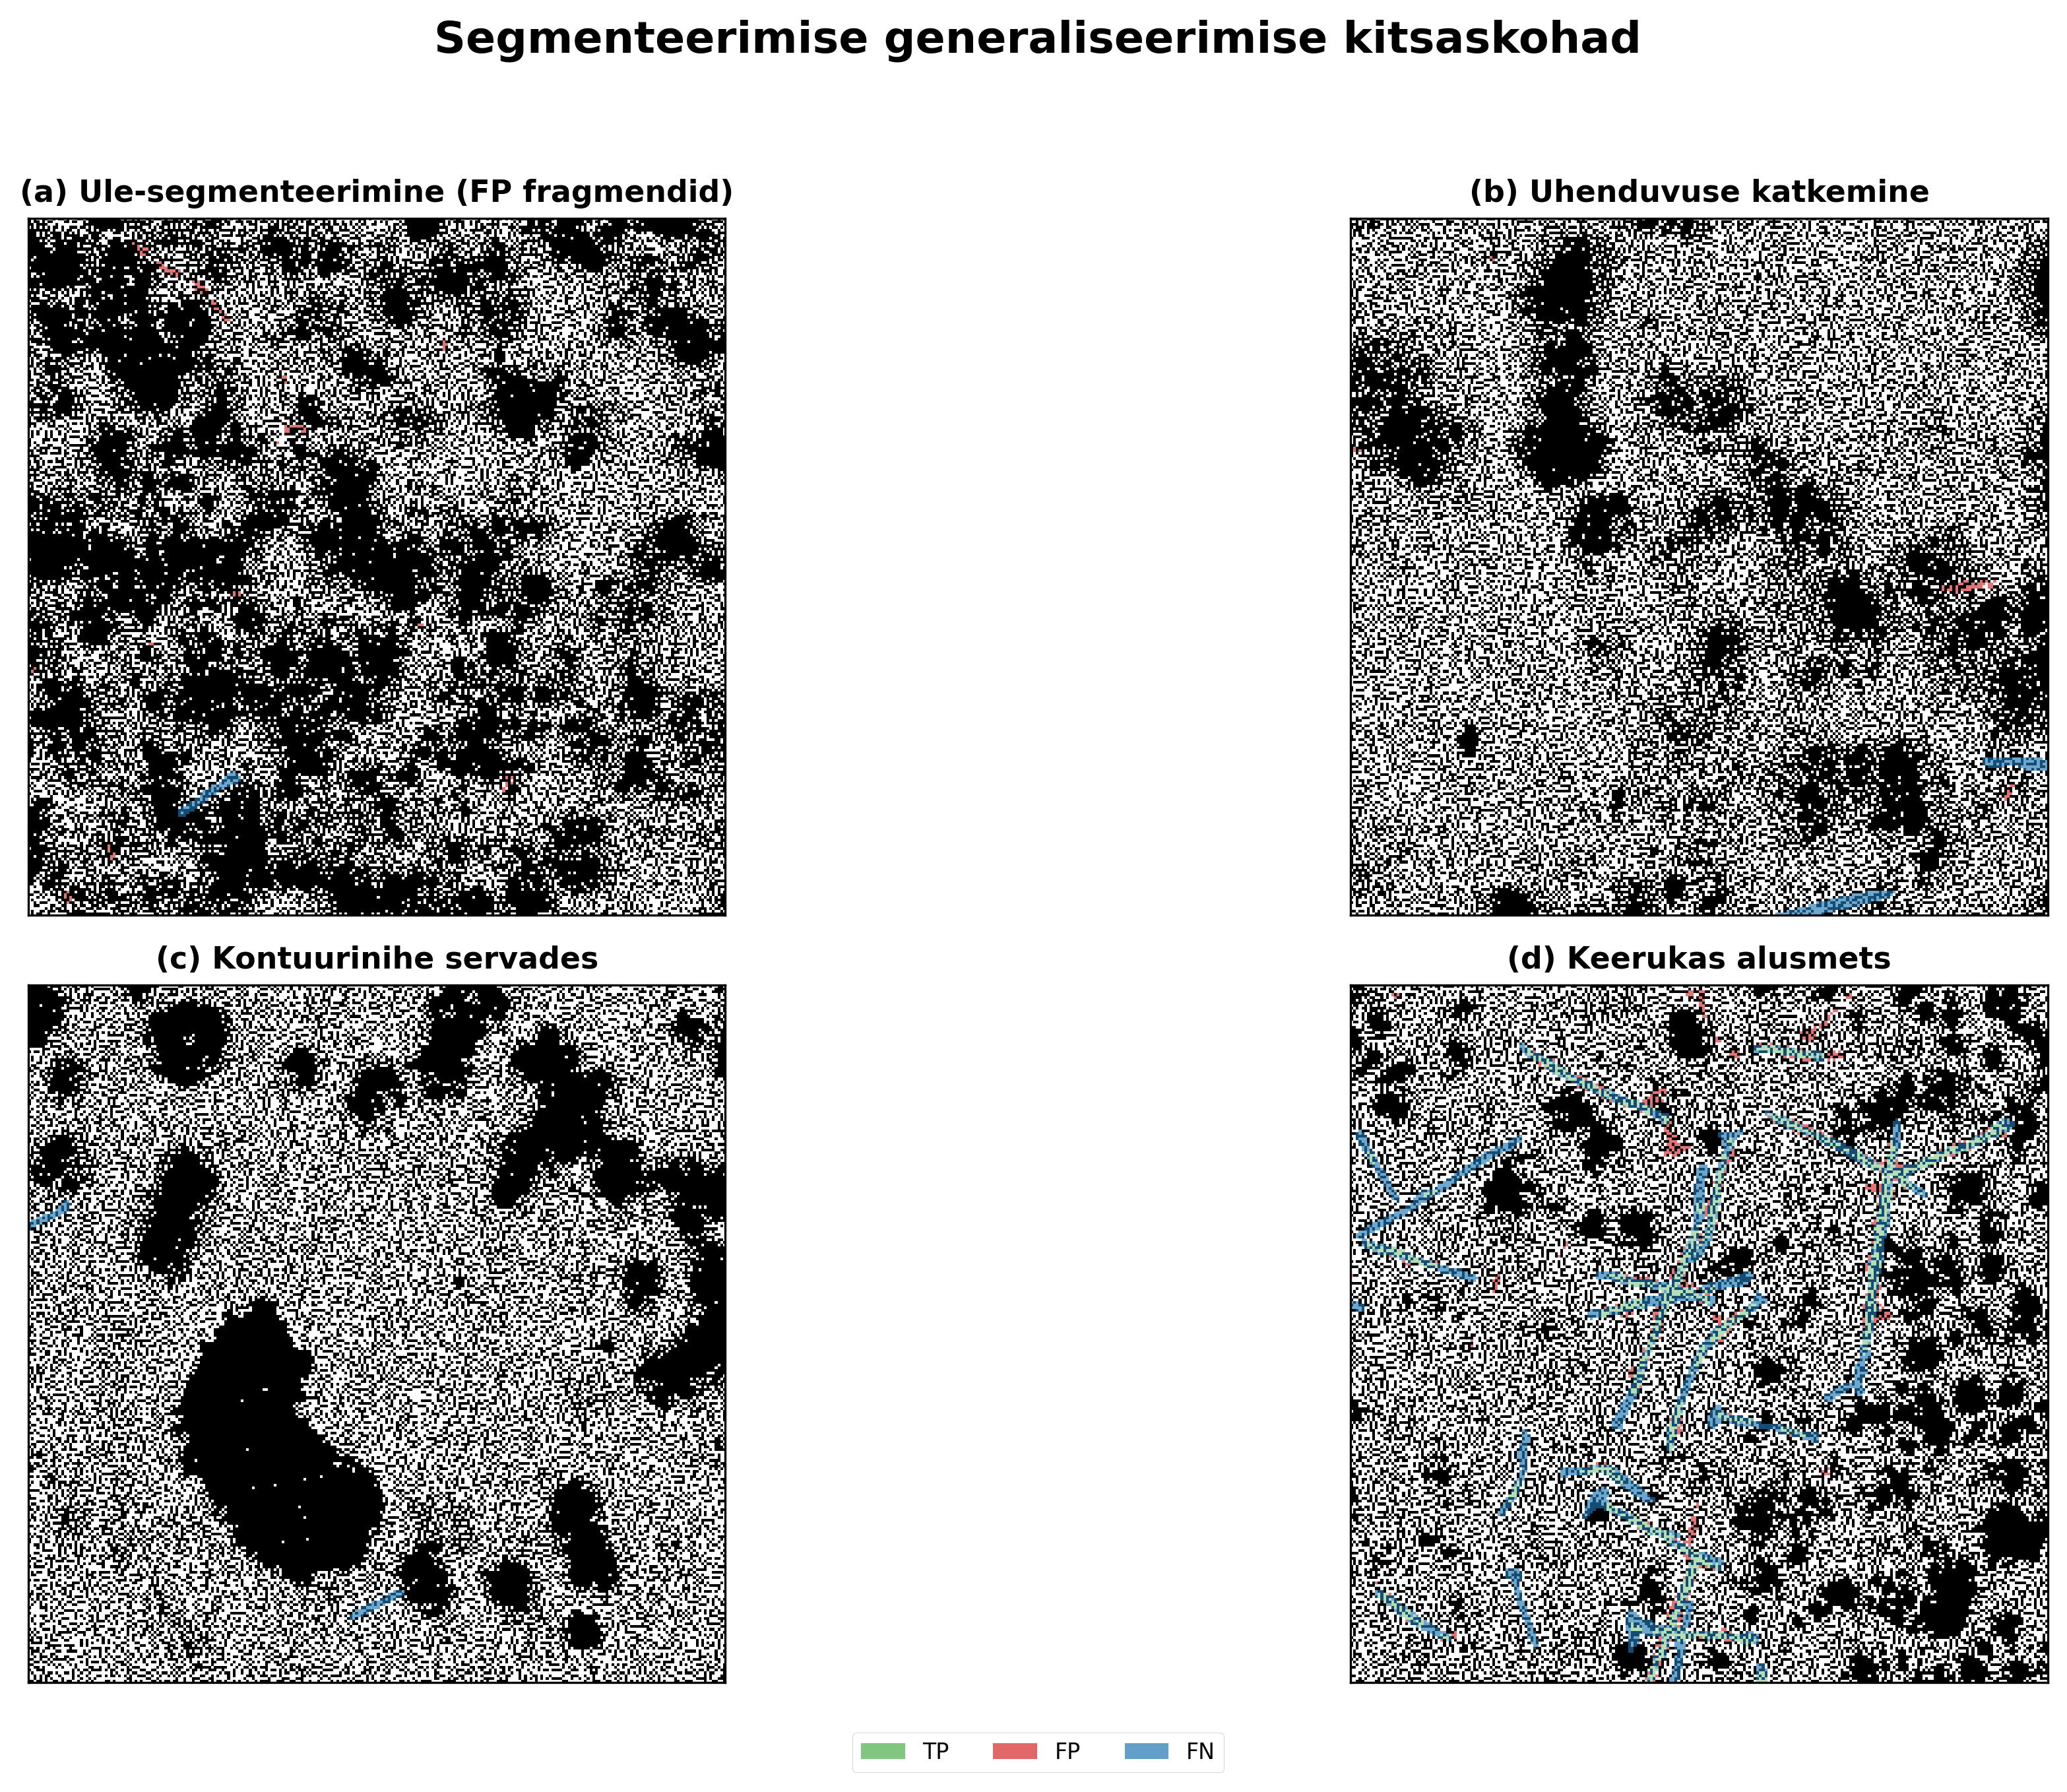
\includegraphics[width=0.95\linewidth]{estonian/joonised/seg_generaliseerimise_kitsaskohad.png}
\caption{Generaliseerimise kitsaskohad eraldiseisvatel testplokkidel.}
\label{fig:seg-error-panel}
\end{figure}

\begin{figure}[h!]
\centering
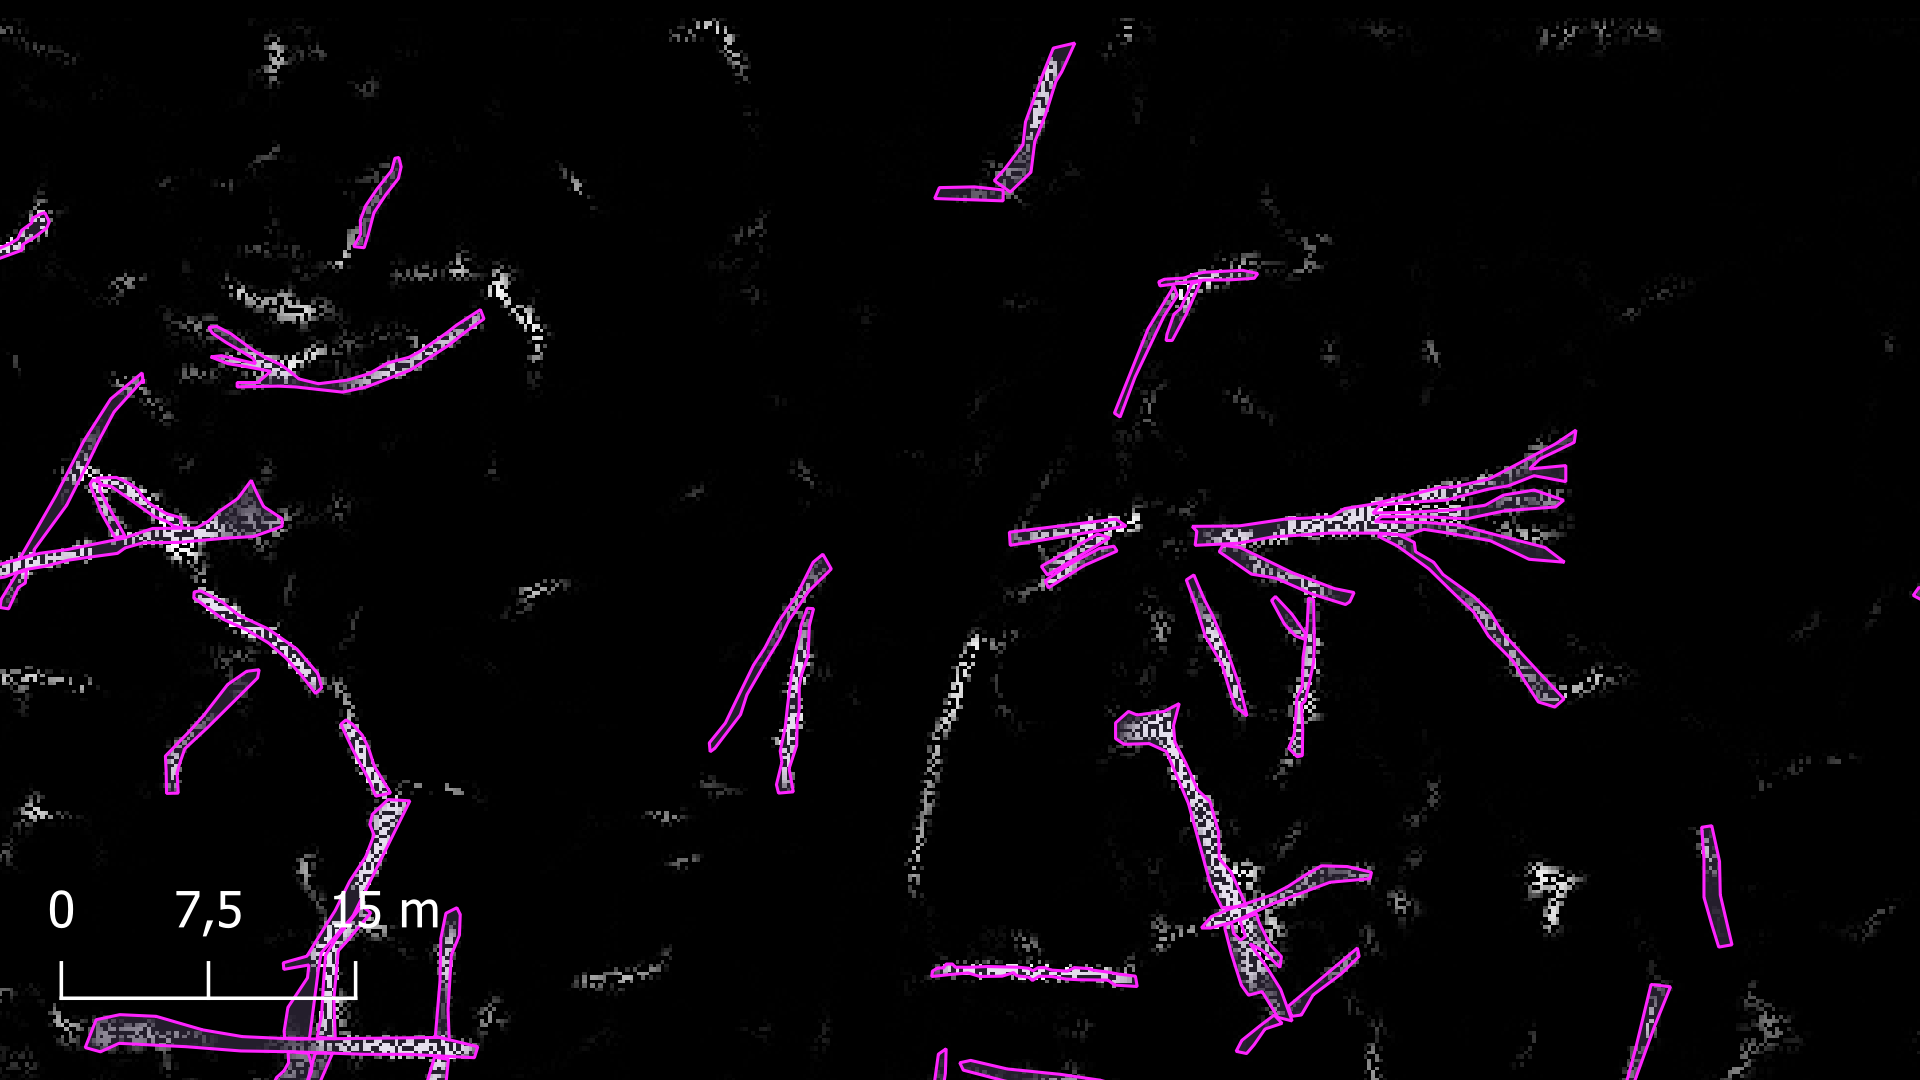
\includegraphics[width=0.95\linewidth]{estonian/joonised/Ruhnu_Prob_tõene.png}
\caption{Segmenteerimise tõenäosus jaotus koos tõeste aladega  (lilla)}
\label{fig:seg-error-panel}
\end{figure}
\newpage
